\subsubsection{Frage 5}
\paragraph{Frage}
Warum zeigt der Packet Tracer bei dem hinzugefügten Link nicht mehr
zwei grüne (also aktive) Ports an?
\paragraph{Antwort}
Weil die Switches im STP Mode sind.Die extra Leitung wird erst dann eingeschaltet, wenn die andere Leitung ausfällt, damit keine switching loops enstehen und die MAC-Tabellen(SATs) nicht ``corrupted'' werden.
\subsubsection{FTP Resultat}
User 192.168.1.1: 15.576 sec\\
User 192.168.1.2: 15.392 sec\\
Admin 192.168.2.1: 15.265 sec\\
Admin 192.168.2.2: 15.265 sec\\
\begin{figure}[!htb]
    \centering
    \begin{subfigure}{.45\textwidth}
        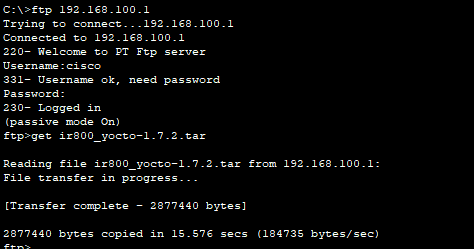
\includegraphics[width=\textwidth,height=\textwidth,keepaspectratio]{./img/tests/User1.png}
        \caption{User 192.168.1.1}
    \end{subfigure}
    \begin{subfigure}{.45\textwidth}
        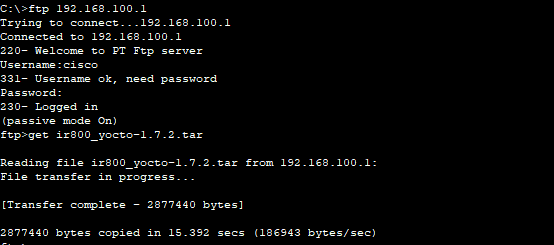
\includegraphics[width=\textwidth,height=\textwidth,keepaspectratio]{./img/tests/User2.png}
        \caption{User 192.168.1.2}
    \end{subfigure}
    ~
    \begin{subfigure}{.45\textwidth}
        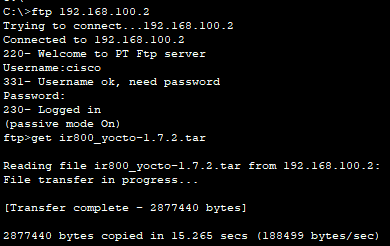
\includegraphics[width=\textwidth,height=\textwidth,keepaspectratio]{./img/tests/Admin1.png}
        \caption{Admin 192.168.2.1}
    \end{subfigure}
    \begin{subfigure}{.45\textwidth}
        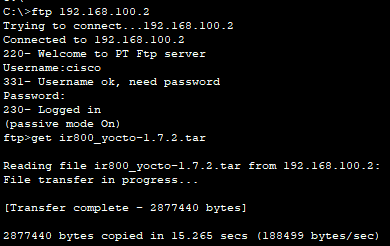
\includegraphics[width=\textwidth,height=\textwidth,keepaspectratio]{./img/tests/Admin1.png}
        \caption{Admin 192.168.2.2}
    \end{subfigure}
\end{figure}